\documentclass[conference]{IEEEtran}
\usepackage{graphicx,booktabs,xcolor,amsmath,amssymb,url,cite,multirow}
\usepackage{algorithm,algpseudocode}
\usepackage{tikz}
\usetikzlibrary{arrows.meta,positioning}
\graphicspath{{../results/figures/}}
\providecommand{\tbd}{\textcolor{red}{\textbf{TBD}}}
\newcommand{\dmMAE}{9.2}
\newcommand{\dmR}{0.60}
\newcommand{\dmRtwo}{0.35}
\newcommand{\dmN}{200}
\newcommand{\hcMAE}{7.4}
\newcommand{\hcR}{0.53}
\newcommand{\hcRtwo}{-1.9}
\newcommand{\biasA}{0.88}
\newcommand{\bagHC}{0.0}
\newcommand{\bagHCsd}{8.7}
\newcommand{\bagAD}{-11.2}
\newcommand{\bagADsd}{14.2}
\newcommand{\bagFTD}{-2.2}
\newcommand{\bagFTDsd}{17.8}
\newcommand{\bagD}{-0.93}
\newcommand{\bagWelchP}{p < 0.001}
\newcommand{\bagMwuP}{p < 0.001}
\newcommand{\bagWelchT}{-3.90}
\newcommand{\bagDci}{[$-1.52$, $-0.46$]}
\newcommand{\bagDiffCI}{[$-16.9$, $-5.6$]}
\newcommand{\bagAUCci}{[$0.56$, $0.82$]}
\newcommand{\bagPermP}{p = 0.002}
\newcommand{\bagAUC}{0.70}
\newcommand{\bagAcc}{66\%}
\newcommand{\bagPrec}{68\%}
\newcommand{\bagRec}{72\%}
\newcommand{\bagSpec}{59\%}
\newcommand{\bagFone}{0.70}
\newcommand{\bagThr}{-2.6}
\newcommand{\ftdHCd}{-0.17}
\newcommand{\ftdHCp}{p = 0.87}
\newcommand{\adFTDd}{-0.57}
\newcommand{\adFTDp}{p = 0.04}
\newcommand{\mmseRho}{-0.08}
\newcommand{\mmseP}{p = 0.62}
\newcommand{\nStable}{12}
\newcommand{\nStableYounger}{12}
\newcommand{\nConfigs}{36}
\newcommand{\stableDlo}{-0.99}
\newcommand{\stableDhi}{-0.26}
\newcommand{\icaD}{-0.70}
\newcommand{\icaP}{p = 0.02}
\newcommand{\repD}{-0.83}
\newcommand{\repAUC}{0.71}
\newcommand{\repPermP}{p = 0.003}
\newcommand{\repHCMAE}{12.6}
\newcommand{\repADFTDp}{p = 0.002}
\newcommand{\repDmMAE}{8.4}
\newcommand{\repDmR}{0.71}
\newcommand{\cnnAUC}{0.89}
\newcommand{\cnnAUCsd}{0.03}
\newcommand{\cnnAcc}{82\%}
\newcommand{\cnnAccsd}{2\%}
\newcommand{\cnnBalAcc}{82\%}
\newcommand{\cnnBalAccsd}{3\%}
\newcommand{\cnnPrec}{84\%}
\newcommand{\cnnPrecsd}{4\%}
\newcommand{\cnnRec}{83\%}
\newcommand{\cnnRecsd}{0\%}
\newcommand{\cnnSpec}{80\%}
\newcommand{\cnnSpecsd}{5\%}
\newcommand{\cnnFone}{0.84}
\newcommand{\cnnFonesd}{0.02}
\newcommand{\cnnAUClo}{0.86}
\newcommand{\cnnAUChi}{0.90}
\newcommand{\cnnPrimAUC}{0.86}
\newcommand{\cnnPrimAUCci}{[$0.76$, $0.94$]}
\newcommand{\cnnPrimAcc}{80\%}
\newcommand{\cnnPrimAccci}{[69, 89]\%}
\newcommand{\cnnPermP}{\tbd{}}
\newcommand{\cnnPermN}{\tbd{}}
\newcommand{\cnnPermNull}{\tbd{}}
\newcommand{\cnnPermNullMax}{\tbd{}}
\newcommand{\cnnFinalEpochs}{3}
\newcommand{\bestModel}{EEGNet (raw EEG)}
\newcommand{\bestModelAUC}{0.88}
\newcommand{\modelAUClo}{0.84}
\newcommand{\modelAUChi}{0.88}
\newcommand{\minDiffP}{0.63}
\newcommand{\combAUC}{0.87}
\newcommand{\combAcc}{78\%}
\newcommand{\combCnnAUC}{0.86}
\newcommand{\combBagAUC}{0.73}
\newcommand{\combDiff}{0.01}
\newcommand{\combDiffCI}{[$-0.06$, $0.08$]}
\newcommand{\combP}{p = 0.74}
\newcommand{\ablFull}{0.89}
\newcommand{\ablSlow}{0.85}
\newcommand{\ablFast}{0.87}
\newcommand{\ablNoTime}{0.84}
\newcommand{\ablEight}{0.85}
\newcommand{\ablSixty}{0.88}
\newcommand{\ablMaxDrop}{0.05}
\newcommand{\mcCNNBalAcc}{63\%}
\newcommand{\mcCNNMacroF}{0.63}
\newcommand{\mcCNNMacroAUC}{0.78}
\newcommand{\mcCNNAcc}{65\%}
\newcommand{\mcRFBalAcc}{56\%}
\newcommand{\mcRFMacroF}{0.55}
\newcommand{\mcRFMacroAUC}{0.72}
\newcommand{\mcRFAcc}{59\%}
\newcommand{\mcRecHC}{76\%}
\newcommand{\mcRecAD}{69\%}
\newcommand{\mcRecFTD}{45\%}
\newcommand{\mcFTDasAD}{10}
\newcommand{\mcNFTD}{22}
\newcommand{\gcOOFADdelta}{0.81}
\newcommand{\gcOOFADtheta}{1.29}
\newcommand{\gcOOFADalpha}{1.27}
\newcommand{\gcOOFADbeta}{1.09}
\newcommand{\gcOOFADgamma}{0.64}
\newcommand{\gcOOFHCdelta}{0.65}
\newcommand{\gcOOFHCtheta}{0.96}
\newcommand{\gcOOFHCalpha}{1.35}
\newcommand{\gcOOFHCbeta}{1.47}
\newcommand{\gcOOFHCgamma}{0.94}
\newcommand{\gcFINALADdelta}{0.83}
\newcommand{\gcFINALADtheta}{1.29}
\newcommand{\gcFINALADalpha}{1.39}
\newcommand{\gcFINALADbeta}{1.07}
\newcommand{\gcFINALADgamma}{0.40}
\newcommand{\gcFINALHCdelta}{0.58}
\newcommand{\gcFINALHCtheta}{1.12}
\newcommand{\gcFINALHCalpha}{1.37}
\newcommand{\gcFINALHCbeta}{1.40}
\newcommand{\gcFINALHCgamma}{1.02}
\newcommand{\gcTopChAD}{F8, T6, T3, P4}
\newcommand{\nDortmund}{200}
\newcommand{\nTarget}{87}
\newcommand{\nAD}{36}
\newcommand{\nHC}{29}
\newcommand{\nFTD}{22}

\makeatletter\newcommand{\tableinput}[1]{\@@input #1 }\makeatother

\begin{document}

\title{When Alzheimer's EEG Does Not Look Old: Brain-Age Gap and CWT-Scalogram CNNs for Interpretable Alzheimer's Disease Detection}

\author{\IEEEauthorblockN{Aayush Soni, Manasa M, Aamal Magdum, Afreen Anz, and Aparna Sankar}
\IEEEauthorblockA{Department of Computer Science and Engineering\\
B.\,M.\,S. College of Engineering, Bengaluru, India}}

\maketitle

% =====================================================================
\begin{abstract}
Resting-state electroencephalography (EEG) is a low-cost candidate for Alzheimer's disease (AD) screening. We present an interpretable EEG pipeline with two complementary modules, evaluated on public data with strictly subject-independent validation. The first is a brain-age model trained only on healthy adults. It was trained on \dmN{} adults aged 20--70 years and transferred to a clinical cohort of \nAD{} AD patients, \nHC{} healthy controls (HC) and \nFTD{} frontotemporal dementia (FTD) patients. The second is a compact convolutional neural network (CNN) on continuous-wavelet-transform (CWT) scalograms, explained with Grad-CAM. Contrary to the accelerated-aging hypothesis, the bias-corrected brain-age gap (BAG) was strongly \emph{negative} in AD ($\bagAD{}\pm\bagADsd{}$ vs. $\bagHC{}\pm\bagHCsd{}$ years in HC; Cohen's $d=\bagD{}$, 95\% CI \bagDci{}). This effect was specific to AD (FTD vs. HC: $d=\ftdHCd{}$). It held across all numerically stable model configurations, on ICA-cleaned data, and in a replication with \repNok{} healthy training subjects. Feature-level analysis explains the reversal: slow-wave power falls and beta power rises with healthy aging, whereas AD shows the opposite. The CNN classified AD vs. HC with AUC \cnnAUC{} and accuracy \cnnAcc{} (mean of three seeds). This was statistically indistinguishable from spectral-feature baselines and EEGNet. Adding the BAG did not improve it ($\Delta$AUC $=\combDiff{}$, \combP{}). Grad-CAM attributed AD decisions mainly to theta and alpha activity. We conclude that EEG brain age in AD reflects a deviation from normative aging rather than accelerated aging.
\end{abstract}

\begin{IEEEkeywords}
Alzheimer's disease, EEG, brain age, continuous wavelet transform, convolutional neural network, Grad-CAM, explainable AI
\end{IEEEkeywords}

% =====================================================================
\section{Introduction}
Alzheimer's disease is the most common cause of dementia. Diagnosis currently relies on clinical assessment, neuropsychological testing and costly imaging such as MRI and PET, which are scarce in resource-limited settings. Resting-state EEG is inexpensive, non-invasive and widely available, and AD alters it in a characteristic way: oscillatory ``slowing'', with more delta and theta and less alpha and beta activity~\cite{jeong2004,babiloni2020}.

Two families of computational methods exploit EEG for AD. \emph{Discriminative classifiers} learn to separate patients from controls directly, using hand-crafted spectral features or deep networks on raw or time--frequency representations~\cite{craik2019,roy2019}. \emph{Brain-age models} are trained only on healthy people to predict chronological age. The brain-age gap (BAG, predicted minus chronological age) is then read as a marker of accelerated aging and has been used widely in neuroimaging~\cite{cole2017,franke2019}. Classifiers often achieve high accuracy but are opaque. Brain age offers an intuitive, continuous score, but its assumption that disease ``ages'' the brain is rarely tested for EEG.

This work combines both approaches in one reproducible pipeline and tests them under strict subject-independent evaluation. Our contributions are:
\begin{enumerate}
\item A harmonized EEG brain-age module trained on healthy adults and transferred to a clinical AD cohort without ever training on patients. We show that the AD brain-age gap is robustly \emph{negative} and AD-specific, and we explain this through opposite spectral changes in aging and AD.
\item A compact CWT-scalogram CNN with Grad-CAM explanations, compared on identical subject folds with four baselines, with ablations and a three-class (HC/AD/FTD) extension.
\item An honest assessment of combining the two modules. The BAG adds interpretability, not accuracy.
\item An open, end-to-end implementation, including an interactive application that produces a per-person report.
\end{enumerate}

% =====================================================================
\section{Related Work}
\subsection{EEG markers of Alzheimer's disease}
Reviews of EEG in AD consistently report slowing of the dominant rhythm, increased delta and theta power, and decreased alpha and beta power. These changes are often accompanied by reduced synchronization~\cite{jeong2004,babiloni2020}. Babiloni et al.\ emphasize that these changes differ from those of normal aging~\cite{babiloni2020}. This distinction is central to our brain-age findings.

\subsection{Machine learning and deep learning on EEG}
Classical pipelines extract band powers or spectral ratios and apply classifiers such as SVMs or random forests. Deep learning removes manual feature design: CNNs on raw signals or on time--frequency images such as spectrograms and wavelet scalograms have been applied to many EEG tasks~\cite{craik2019,roy2019}. EEGNet is a widely used compact architecture for raw EEG~\cite{eegnet}. Reviews caution that small datasets and subject-dependent splits often inflate reported accuracy~\cite{roy2019,varoquaux2018}. For this reason we use subject-level splits and strong baselines throughout.

\subsection{Brain age}
Brain-age prediction from MRI is an established biomarker framework~\cite{cole2017,franke2019}. Statistical bias toward the mean age must be corrected~\cite{delange2020}. EEG-based brain age has been estimated from resting-state recordings~\cite{alzoubi2018,engemann2022}. Sleep-EEG brain age was elevated in people with dementia~\cite{sun2019}, supporting the accelerated-aging view. Whether this holds for resting-state EEG in clinically diagnosed AD, using a model that never sees patients, has not been established.

\subsection{Explainability and harmonization}
Grad-CAM produces class-specific importance maps from the last convolutional layer of a CNN~\cite{gradcam}. On scalograms these maps can be read as frequency-by-time importance. Combining data from different sites requires harmonization; ComBat~\cite{johnson2007} removes site effects while protecting biological covariates and has been adopted for neuroimaging~\cite{fortin2018}.

% =====================================================================
\section{Proposed Methodology}
Fig.~\ref{fig:pipeline} summarizes the system. One harmonized preprocessing stage feeds two modules: a brain-age module trained on healthy adults, and a CWT-scalogram CNN classifier. Their outputs are reported side by side and can be combined.

\begin{figure}[t]
\centering
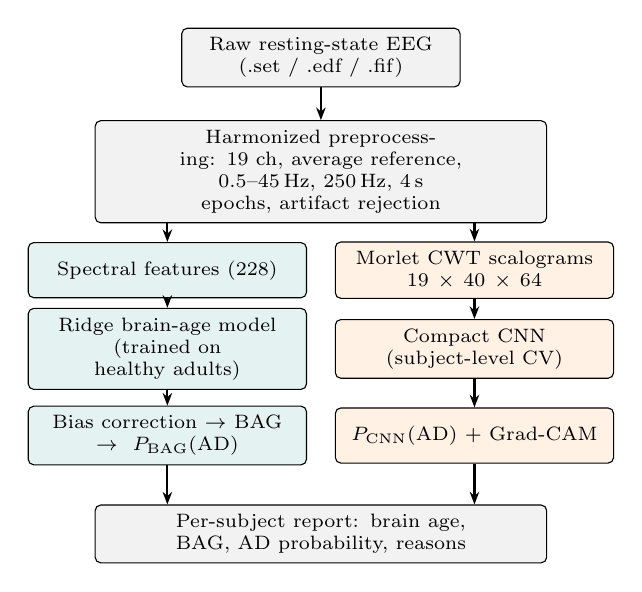
\begin{tikzpicture}[every node/.style={font=\scriptsize},
  box/.style={draw, rounded corners=2pt, align=center, minimum height=7mm, text width=3.3cm, fill=#1!10},
  box/.default=gray, ar/.style={-{Stealth[length=1.6mm]}, thick}]
\node[box=gray] (raw) at (0,0.45) {Raw resting-state EEG (.set / .edf / .fif)};
\node[box=gray, text width=5.5cm] (pre) at (0,-1.0) {Harmonized preprocessing: 19 ch, average reference,\\0.5--45\,Hz, 250\,Hz, 4\,s epochs, artifact rejection};
\node[box=teal] (feat) at (-1.95,-2.25) {Spectral features (228)};
\node[box=teal] (ba) at (-1.95,-3.25) {Ridge brain-age model\\(trained on healthy adults)};
\node[box=teal] (bag) at (-1.95,-4.35) {Bias correction $\rightarrow$ BAG\\$\rightarrow P_\mathrm{BAG}(\mathrm{AD})$};
\node[box=orange] (cwt) at (1.95,-2.25) {Morlet CWT scalograms\\$19\times40\times64$};
\node[box=orange] (cnn) at (1.95,-3.25) {Compact CNN\\(subject-level CV)};
\node[box=orange] (gc) at (1.95,-4.35) {$P_\mathrm{CNN}(\mathrm{AD})$ + Grad-CAM};
\node[box=gray, text width=5.5cm] (rep) at (0,-5.6) {Per-subject report: brain age, BAG, AD probability, reasons};
\draw[ar] (raw) -- (pre); \draw[ar] (pre.south) ++(-1.95,0) -- (feat); \draw[ar] (pre.south) ++(1.95,0) -- (cwt);
\draw[ar] (feat) -- (ba); \draw[ar] (ba) -- (bag); \draw[ar] (cwt) -- (cnn); \draw[ar] (cnn) -- (gc);
\draw[ar] (bag.south) -- (bag.south |- rep.north); \draw[ar] (gc.south) -- (gc.south |- rep.north);
\end{tikzpicture}
\caption{Proposed pipeline. Teal: brain-age module. Orange: CNN classifier.}
\label{fig:pipeline}
\end{figure}

\subsection{Harmonized preprocessing}
A single function processes training data, test data and new uploads, using MNE-Python~\cite{mne}. It selects 19 channels in a fixed order (10--10 names mapped to 10--20), applies an average reference over these channels, a 0.5--45\,Hz zero-phase FIR band-pass and resampling to 250\,Hz. It then cuts 4\,s epochs with 2\,s overlap and rejects epochs whose peak-to-peak amplitude exceeds 150\,$\mu$V or falls below 1\,$\mu$V. ICA is not applied, so the pipeline is identical across datasets and deployment. The effect of this choice is tested with the dataset authors' ICA-cleaned data.

\subsection{Brain-age module}
For each subject, the Welch power spectrum (4\,s Hann window) is averaged over epochs. From it we compute per channel: log absolute and relative power in the delta (1--4\,Hz), theta (4--8), alpha (8--13) and beta (13--30\,Hz) bands; the alpha peak frequency; the log theta/alpha ratio; and the aperiodic exponent and offset (FOOOF~\cite{fooof}). This gives 228 features. A ridge regressor predicts age. Because the clinical cohort spans a narrow age range, ds004504 HC are added to the healthy training set, and every HC prediction is made out-of-fold. Age bias is corrected on HC predictions~\cite{delange2020}, and the BAG is mapped to $P(\mathrm{AD})$ with logistic regression. \textbf{AD and FTD subjects never enter training, harmonization or model selection.}

\subsection{CWT-scalogram CNN}
Each epoch becomes a Morlet scalogram with 40 log-spaced frequencies (1--40\,Hz) and 64 time bins, a $19\times40\times64$ tensor with EEG channels as input feature maps. The CNN has three blocks of convolution ($3\times3$), batch normalization and ReLU (16, 32 and 32 filters, the first two followed by max-pooling), then global average pooling, dropout of 0.5 and a linear output. It has about 17k parameters, deliberately small for a 65-subject cohort. A subject's probability is the mean over its epochs. Grad-CAM~\cite{gradcam} on the last block yields frequency-by-time importance.

\subsection{Combination and evaluation protocol}
The two modules are combined by stacking: logistic regression on $[\mathrm{logit}\,P_\mathrm{CNN},\,\mathrm{BAG}]$. All evaluation is subject-independent. The CNN uses subject-level 10-fold cross-validation repeated with three seeds, each changing both the fold split and the initialization. Baselines use identical folds. We report AUC, accuracy, precision, recall, specificity and F1, with 95\% bootstrap CIs (2000 subject resamples). AUC significance is assessed by permutation tests that re-run the entire CV on shuffled labels~\cite{ojala2010}, and model differences by a paired bootstrap.

% =====================================================================
\section{Algorithms}

\begin{algorithm}[t]
\caption{Harmonized preprocessing}
\label{alg:pre}
\begin{algorithmic}[1]
\Require EEG recording $R$; channel list $\mathcal{C}$ (19, 10--20)
\Ensure clean epochs $X \in \mathbb{R}^{n\times19\times1000}$
\State map 10--10 names (T7, T8, P7, P8) to 10--20 (T3, T4, T5, T6)
\If{any channel of $\mathcal{C}$ is missing or duration $< 30$\,s} \State \textbf{reject} with an explanatory message \EndIf
\State select $\mathcal{C}$ in fixed order; re-reference to their average
\State band-pass 0.5--45\,Hz (zero-phase FIR); resample to 250\,Hz
\State cut 4\,s epochs with 2\,s overlap
\State keep epoch $e$ iff $1\,\mu\mathrm{V} < \mathrm{ptp}_c(e) < 150\,\mu\mathrm{V}$ for all channels $c$
\If{fewer than 10 epochs remain} \State \textbf{reject} \EndIf
\State \Return $X$ (cached by configuration hash)
\end{algorithmic}
\end{algorithm}

\begin{algorithm}[t]
\caption{Brain-age training, transfer and BAG}
\label{alg:ba}
\begin{algorithmic}[1]
\Require healthy cohort $D_H$ (age 20--70); target HC set $T_C$; patients $T_P$ (AD, FTD)
\Ensure BAG for every target subject
\For{each $s \in T_C$} \Comment{leave-one-HC-out}
  \State fit ridge (inner-CV $\alpha$) on features of $D_H \cup T_C\setminus\{s\}$
  \State $\hat{y}_s \gets$ predicted age of $s$
\EndFor
\State fit ridge on $D_H \cup T_C$; $\hat{y}_p \gets$ prediction for each $p \in T_P$
\State fit $\hat{y} = a\,y + b$ on $\{(y_s,\hat{y}_s): s\in T_C\}$ \Comment{HC only}
\State $\mathrm{BAG}_i \gets (\hat{y}_i - b)/a - y_i$ for all target subjects $i$
\State \Return BAG; fit $P(\mathrm{AD}\mid\mathrm{BAG})$ by logistic regression
\end{algorithmic}
\end{algorithm}

\begin{algorithm}[t]
\caption{Subject-level cross-validation of the CNN}
\label{alg:cnn}
\begin{algorithmic}[1]
\Require subjects $S$ with labels; scalograms $Z_s$ ($\le150$ per subject); seed $r$
\Ensure out-of-fold $P(\mathrm{AD})$ for every subject
\State split $S$ into 10 stratified folds $F_1,\dots,F_{10}$ (seed $r$)
\For{$k = 1$ to $10$}
  \State $S_\mathrm{tr} \gets S \setminus F_k$; split $S_\mathrm{tr}$ into fit (85\%) and validation (15\%) subjects
  \State compute mean/SD per channel$\times$frequency on fit subjects only
  \State train CNN on fit epochs (Adam, weighted BCE)
  \State stop when validation-subject loss has not improved for 6 epochs; restore best weights
  \For{each $s \in F_k$} \State $P_s \gets$ mean of epoch probabilities of $s$ \EndFor
\EndFor
\State \Return $\{P_s\}$ \Comment{no subject is in both training and test}
\end{algorithmic}
\end{algorithm}

\begin{algorithm}[t]
\caption{Inference for a new subject}
\label{alg:inf}
\begin{algorithmic}[1]
\Require EEG file, chronological age $y$
\State $X \gets$ Algorithm~\ref{alg:pre}(file)
\State brain age $\hat{y} \gets$ ridge(features($X$)); $\mathrm{BAG} \gets (\hat{y}-b)/a - y$
\State $P_\mathrm{CNN} \gets$ mean CNN probability over scalograms of $X$
\State Grad-CAM band importance toward the predicted class
\State compare alpha peak, band ratios and BAG with HC/AD reference values
\State \Return report: brain age, BAG, $P_\mathrm{CNN}$, $P_\mathrm{BAG}$, combined $P$, reasons
\end{algorithmic}
\end{algorithm}

Algorithms~\ref{alg:pre}--\ref{alg:inf} specify the pipeline. Algorithm~\ref{alg:ba} guarantees that no patient influences the age model or its bias correction. Algorithm~\ref{alg:cnn} guarantees that normalization, early stopping and testing never share subjects. Algorithm~\ref{alg:inf} runs in about 10\,s per recording on a laptop CPU.

% =====================================================================
\section{Dataset}
\emph{Clinical cohort (OpenNeuro ds004504)}~\cite{miltiadous2023}. Resting-state eyes-closed EEG from \nAD{} AD, \nHC{} HC and \nFTD{} FTD subjects aged roughly 44--79, recorded clinically with 19 electrodes (10--20 system) at 500\,Hz. Labels include MMSE scores. One FTD recording failed artifact screening. The authors also provide ICA-cleaned derivatives, which we used only for sensitivity analysis. The dataset contains no mild-cognitive-impairment subjects, so the classification task is AD vs. HC, with FTD as an additional class.

\emph{Healthy aging cohort (OpenNeuro ds005385, Dortmund Vital Study)}~\cite{gajewski2022}. 64-channel EEG at 1000\,Hz from healthy adults aged 20--70. We used the baseline session, eyes-closed, pre-task recordings. Recordings flagged as possibly discontinuous were excluded. The main analysis used an age-stratified sample weighted toward older ages ($n=\dmN{}$; 25/25/35/50/65 per decade); a replication used all \repNsel{} eligible subjects (\repNok{} after preprocessing).

After preprocessing, the clinical subjects kept on average about 80\% of their epochs, and the healthy cohort about 90\%. The median peak-to-peak amplitude was similar in the two cohorts, which confirms consistent units and scaling.

% =====================================================================
\section{Results}
\subsection{Brain age: AD departs from the healthy-aging pattern}
On the healthy cohort the brain-age model reached MAE \dmMAE{} years ($r=\dmR{}$) in 10-fold CV. On ds004504 HC the out-of-fold MAE was \hcMAE{} years ($r=\hcR{}$, bias slope $a=\biasA{}$). The out-of-fold $R^2$ was $\hcRtwo{}$, which is expected for an HC age range of only 57--78 years, so $R^2$ is not used as the success criterion. The bias-corrected BAG was $\bagHC{}\pm\bagHCsd{}$ years in HC, $\bagAD{}\pm\bagADsd{}$ in AD and $\bagFTD{}\pm\bagFTDsd{}$ in FTD (Fig.~\ref{fig:bag}). AD differed from HC (Welch $t=\bagWelchT{}$, \bagWelchP{}; Mann--Whitney \bagMwuP{}; $d=\bagD{}$, 95\% CI \bagDci{}). FTD did not differ from HC ($d=\ftdHCd{}$, \ftdHCp{}), and AD differed from FTD ($d=\adFTDd{}$, \adFTDp{}). The negative AD gap appeared in \nStableYounger{} of \nStable{} numerically stable configurations ($d$ from $\stableDlo{}$ to $\stableDhi{}$). It persisted on ICA-cleaned data ($d=\icaD{}$, \icaP{}) and in the \repNok{}-subject replication ($d=\repD{}$, permutation \repPermP{}). Within AD, BAG was not associated with MMSE ($\rho=\mmseRho{}$, \mmseP{}).

\begin{figure}[t]
\centering
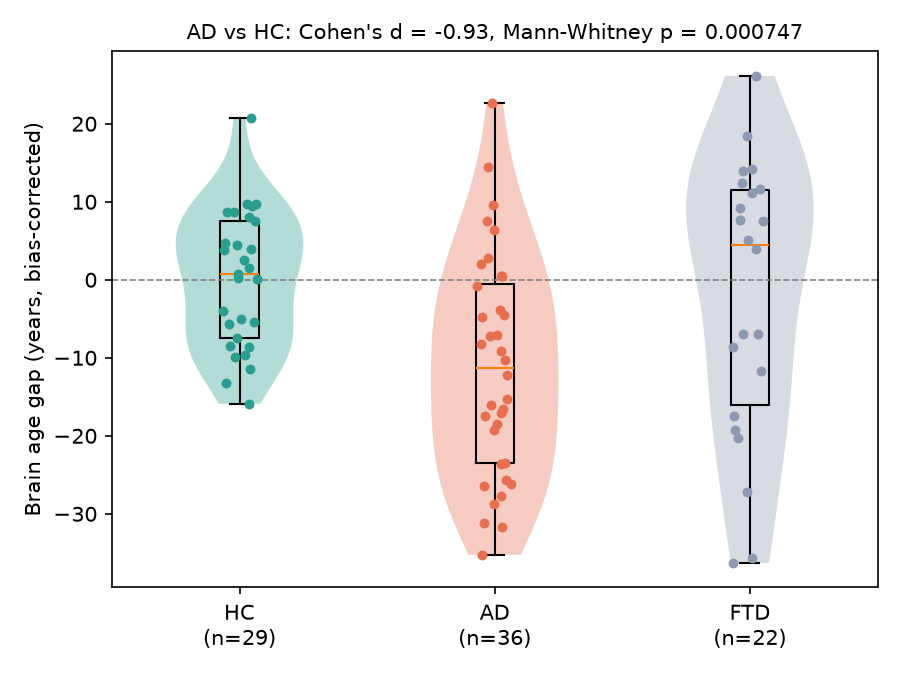
\includegraphics[width=0.92\columnwidth]{bag_by_group.png}
\caption{Bias-corrected brain-age gap by group. HC are out-of-fold; AD and FTD were never used for training.}
\label{fig:bag}
\end{figure}

Table~\ref{tab:dir} explains the reversal. Alpha peak frequency, alpha power and the theta/alpha ratio change in the same direction in aging and AD. In contrast, beta power rises with age but falls in AD, while absolute slow-wave power and the aperiodic exponent fall with age but rise in AD. A model of healthy aging therefore places AD EEG off, and on balance ``before'', the normative trajectory. Used alone as a classifier, BAG reached AUC \bagAUC{} (95\% CI \bagAUCci{}, permutation \bagPermP{}), accuracy \bagAcc{}, precision \bagPrec{}, recall \bagRec{} and specificity \bagSpec{}, with the decision rule BAG $<\bagThr{}$ years.

\begin{table}[t]
\centering
\caption{Healthy-aging direction vs. AD effect per feature family}
\label{tab:dir}
\footnotesize\setlength{\tabcolsep}{4pt}
\begin{tabular}{lccc}
\toprule
Feature & $r$ (age, healthy) & $d$ (AD$-$HC) & AD looks \\
\midrule
\tableinput{generated/table_directions.tex}
\bottomrule
\end{tabular}
\end{table}

\subsection{CNN classification and baselines}
Over three seeds the CNN achieved AUC \cnnAUC{} (range \cnnAUClo{}--\cnnAUChi{}), accuracy \cnnAcc{}, precision \cnnPrec{}, recall \cnnRec{}, specificity \cnnSpec{} and F1 \cnnFone{}. For the primary seed the AUC was \cnnPrimAUC{} (95\% CI \cnnPrimAUCci{}) and the accuracy \cnnPrimAcc{} (95\% CI \cnnPrimAccci{}). In a permutation test with $N=\cnnPermN{}$ full re-runs on shuffled labels, the null AUC averaged \cnnPermNull{} (maximum \cnnPermNullMax{}), giving \cnnPermP{}. On identical folds (Table~\ref{tab:base}) all models performed comparably (AUC \modelAUClo{}--\modelAUChi{}; highest: \bestModel{}, \bestModelAUC{}). No difference from the CNN was significant (all $p \geq \minDiffP{}$). With $n=65$, models within about 0.1 AUC cannot be distinguished~\cite{varoquaux2018}.

\begin{table*}[t]
\centering
\caption{AD vs. HC on identical subject-level 10-fold splits (primary seed, $n=65$). Last column: CNN AUC minus model AUC (paired bootstrap).}
\label{tab:base}
\begin{tabular}{lcccccc}
\toprule
Model & AUC & Acc. (\%) & Recall (\%) & Spec. (\%) & F1 & $\Delta$AUC (CNN$-$model) \\
\midrule
\tableinput{generated/table_baselines.tex}
\bottomrule
\end{tabular}
\end{table*}

\subsection{Combining the two modules}
Stacking the CNN with BAG gave AUC \combAUC{} versus \combCnnAUC{} for the CNN alone ($\Delta=\combDiff{}$, 95\% CI \combDiffCI{}, \combP{}). Both modules draw on the same EEG slowing, so the BAG adds interpretability rather than accuracy.

\subsection{Ablations}
Table~\ref{tab:abl} varies one design choice at a time (three seeds each). No change reduced the mean AUC by more than \ablMaxDrop{}, which is comparable to the variation between seeds. Using only 8--40\,Hz (AUC \ablFast{}) kept more information than using only 1--8\,Hz (\ablSlow{}), and collapsing the time axis (\ablNoTime{}) gave a small drop. Eight channels (\ablEight{}) and 40\% of the epochs (\ablSixty{}) stayed close to the full model (\ablFull{}). This suggests that low-density montages and shorter recordings are viable.

\begin{table}[t]
\centering
\caption{CNN ablations (mean $\pm$ SD over seeds)}
\label{tab:abl}
\footnotesize\setlength{\tabcolsep}{3pt}
\begin{tabular}{lccc}
\toprule
Variant & AUC & Acc. (\%) & seeds \\
\midrule
\tableinput{generated/table_ablation.tex}
\bottomrule
\end{tabular}
\end{table}

\subsection{Three-class classification}
For HC/AD/FTD the CNN reached balanced accuracy \mcCNNBalAcc{} (macro AUC \mcCNNMacroAUC{}), versus \mcRFBalAcc{} (\mcRFMacroAUC{}) for a random forest on spectral features. Class recall was \mcRecHC{} for HC, \mcRecAD{} for AD and \mcRecFTD{} for FTD; \mcFTDasAD{} of \mcNFTD{} FTD subjects were classified as AD (Table~\ref{tab:conf3}). This is consistent with the overlapping EEG slowing of the two dementias.

\begin{table}[t]
\centering
\caption{Three-class CNN confusion matrix (primary seed; rows: true class)}
\label{tab:conf3}
\begin{tabular}{lccc}
\toprule
True $\backslash$ predicted & HC & AD & FTD \\
\midrule
\tableinput{generated/table_confusion3.tex}
\bottomrule
\end{tabular}
\end{table}

\subsection{Explainability}
Relative to the average over frequencies (1.0), final-model Grad-CAM importance for AD decisions was theta \gcFINALADtheta{}, alpha \gcFINALADalpha{}, delta \gcFINALADdelta{} and beta \gcFINALADbeta{}. For HC decisions it was alpha \gcFINALHCalpha{} and beta \gcFINALHCbeta{} (Fig.~\ref{fig:gradcam}). Out-of-fold Grad-CAM, from fold models that never saw the explained subject, reproduced this pattern: AD theta \gcOOFADtheta{} and alpha \gcOOFADalpha{}, and HC alpha \gcOOFHCalpha{} and beta \gcOOFHCbeta{}. The most important channels for AD were temporo-parietal (\gcTopChAD{}). This agrees with the known theta increase and alpha decrease in AD.

\begin{figure*}[t]
\centering
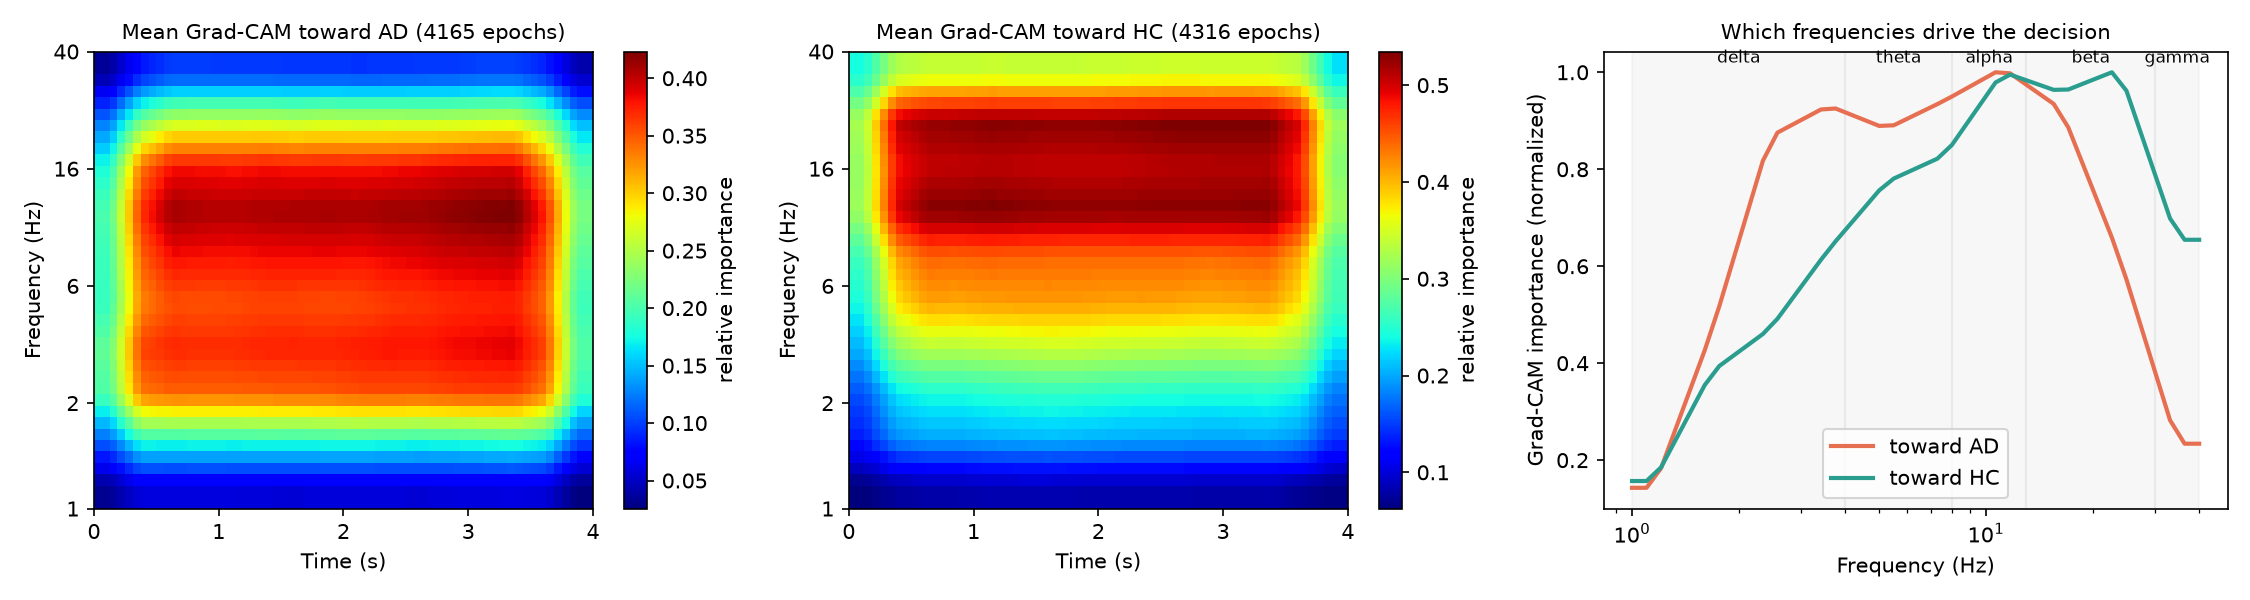
\includegraphics[width=0.9\textwidth]{cnn_gradcam.png}
\caption{Grad-CAM of the final CNN: mean maps toward AD and HC, and frequency profiles.}
\label{fig:gradcam}
\end{figure*}

% =====================================================================
\section{Conclusion and Contribution}
This work tested two interpretable EEG approaches to Alzheimer's disease under strictly subject-independent evaluation on public data. Its contributions and conclusions are:

\emph{1) The brain-age gap in AD is a deviation, not acceleration.} A brain-age model that never saw patients found AD EEG \emph{younger}, not older ($d=\bagD{}$). The effect was AD-specific, robust across configurations, preprocessing and training sets, and explained by spectral features that change in opposite directions in aging and AD. EEG brain age in AD should therefore be interpreted as a normative-deviation score.

\emph{2) A compact, explainable CNN.} The CWT-scalogram CNN reached AUC \cnnAUC{}, above the 0.75 target, with Grad-CAM explanations centred on theta and alpha. It was statistically indistinguishable from spectral baselines and EEGNet, which is a realistic picture for small EEG cohorts.

\emph{3) The value of combining the modules lies in interpretability.} The BAG did not improve classification, but it provides a continuous, explainable score. Both are delivered in a per-subject report by an open application.

\emph{Limitations and future work.} The cohort is small ($n=65$ for AD vs. HC) and there is no external test set. The healthy cohort ends at 70 years, while the clinical HC reach 78. ICA was not used in the main pipeline. BAG did not track MMSE, and the data contain no MCI subjects, so progression could not be studied. Future work will validate the pipeline on independent cohorts, extend it to MCI and longitudinal data, and explore normative modeling of EEG spectra.

\section*{Acknowledgment}
The authors thank Prof.~Manasa, Department of Computer Science and Engineering, B.\,M.\,S. College of Engineering, for her guidance and supervision, and the investigators of OpenNeuro ds004504 and ds005385 for making their data publicly available. AI assistance (Claude, Anthropic) was used for code development and manuscript drafting; the authors verified all results and take full responsibility for the content.

\bibliographystyle{IEEEtran}
\bibliography{refs}

\end{document}
